%% 04b_results_identity.tex -- split from main.tex by paper-planner (2026-10-01). Owner group: G4.
%% Camera-ready rewrite (G4, 2026-10-01). Headline rule: only matched-NFE comparisons in
%% openers and captions; every search number names its selector and its scorer.
\begin{table}[t]
  \centering\small
  \caption{Search against refinement at matched NFE (\NmencRuns\ runs, \NmencItems\ items). Each candidate is
  drawn at $T{=}8$ (64 NFE), so NFE $=64K$. WER is absolute, for the WavLM-L-selected output.}
  \label{tab:search}
  \setlength{\tabcolsep}{4pt}
  \begin{tabular}{rcccccc}
    \toprule
    & & \multicolumn{2}{c}{WavLM-L selects, ECAPA scores}
      & \multicolumn{2}{c}{ECAPA selects, WavLM-L scores} & WER \\
    \cmidrule(lr){3-4}\cmidrule(lr){5-6}
    NFE & $T$ vs $K$ & $\Delta$ similarity & 95\% CI & $\Delta$ SIM-o & 95\% CI
      & refinement / search \\
    \midrule
    128 & 16 vs 2 & \NcrMatchLod  & \NcrMatchLoci  & \NcrXEWLod  & \NcrXEWLoci  & \NsrchLorw\ / \NsrchLosw \\
    256 & 32 vs 4 & \NcrMatchMidd & \NcrMatchMidci & \NcrXEWMidd & \NcrXEWMidci & \NsrchMidrw\ / \NsrchMidsw \\
    512 & 64 vs 8 & \NcrMatchHid  & \NcrMatchHici  & \NcrXEWHid  & \NcrXEWHici  & \NsrchHirw\ / \NsrchHisw \\
    \bottomrule
  \end{tabular}
\end{table}

\subsection{Search raises identity at matched NFE}
\label{sec:search}
At every matched-NFE tier we tested, best-of-$K$ search gives higher speaker similarity than
refinement, and refinement gives lower WER (Table~\ref{tab:search}). At NFE 128, best-of-2
search beats the default $T{=}16$ by \NcrMatchLod\ in ECAPA similarity (CI \NcrMatchLoci)
and wins on \NcrMatchLowin\% of items, with WavLM-L as the selector. With the roles swapped,
so that ECAPA selects and WavLM-L scores, search gains \NcrXEWLod\ in SIM-o (CI
\NcrXEWLoci) and wins on \NcrXEWLowin\% of items. Selecting and scoring with the same
encoder would be circular, so we always use two different ones.

Both pairings of selector and scorer beat refinement at every NFE we tested, and search wins
on more than half of the items in each case (95\% intervals in App.~\ref{app:search}); the
gains are smaller when ECAPA selects. The two selectors pick the same
candidate on only \NcrAgreeLo\%, \NcrAgreeMid\% and \NcrAgreeHi\% of items at $K=2, 4, 8$
(chance: \NcrChanceLo\%, \NcrChanceMid\%, \NcrChanceHi\%). At NFE 512, the four speaker
encoders other than the selector all prefer search, on \NmencLo--\NmencHi\% of items.

Search has two costs. First, it raises WER: the best-of-2 output picked by WavLM-L has
\NcrLedgerSearchWER\ higher absolute WER than $T{=}16$ refinement. More candidates do not
lower it; more refinement steps do (Table~\ref{tab:search}).
Second, selection costs compute, because every candidate is decoded by Mimi and embedded by
WavLM-L. At $K{=}2$ this adds \NcrCostTwopct\% to the FLOPs of generation, as much as
\NcrCostTwonfe\ generator passes. It is at most \NcrCostTwobound\% if phoneme tokens are not
counted, and the estimated CPU wall time is \NcrWallTworatio\ that of refinement. ECAPA and the ASR are used
only for evaluation and add nothing. Refinement given more total compute than search still
loses: best-of-2 beats $T{=}32$ by \NcrEqualTwod\ (App.~\ref{app:search}).

The gap grows to \NcrMatchMidd\ at NFE 256 and \NcrMatchHid\ at NFE 512, partly because
refinement itself gets worse past $T{=}16$: its ECAPA similarity changes by $\NcrRefineDropThirtyTwo$ from $T{=}16$ to $T{=}32$ and by
$\NcrRefineDropSixtyFour$ to $T{=}64$. The NFE 512 result holds on the \NmaxNfour\,M budget
(\NscopeDd; \NcrXEWDd\ with ECAPA selecting) and after $3\times$ training (\NscopeNd;
\NcrXEWNd). At NFE 128 after $3\times$ training, search still gains \NcrXWENLod\ with WavLM-L
selecting, but the swapped control's interval includes zero (\NcrXEWNLod, CI $\NcrXEWNLoci$,
\NcrXNRuns\ runs; App.~\ref{app:search}).

\begin{table}[t]
  \centering\small
  \caption{SIM-o gain (WavLM-L) from each lever, against the headroom left between our best
  90k-step model and the codec ceiling. Each row is one bar of Fig.~\ref{fig:ledger}A. Costs
  are in WER points (one point is 0.01 absolute WER).}
  \label{tab:ledger}
  \setlength{\tabcolsep}{5pt}
  \begin{tabular}{lllc}
    \toprule
    lever & change & cost & $\Delta$ SIM-o \\
    \midrule
    % \NcrLedgerRefine (numbers_cr_extra.tex) is the figure bar's value at its 4 decimals.
    refinement$^{a}$ & $T{=}1 \to 16$ & $16\times$ NFE & \NcrLedgerRefine \\
    training & 30k $\to$ 90k steps & $3\times$ training steps & \NtrainGainSim \\
    parameters & best shape, 20\,M $\to$ \NmaxNfour\,M & larger model & \NparamGainSim \\
    search$^{b}$ & best-of-2 vs $T{=}16$, matched NFE
      & \NcrLedgerSearchWERpts$^{c}$, +\NcrCostTwopct\% compute & \NcrLedgerSearch \\
    search$^{b}$ & best-of-8 vs $T{=}64$, matched NFE
      & \NcrLedgerSearchMatchEightWERpts$^{c}$ & \NcrXEWHid \\
    guidance & $\gamma{=}0.5$ at $T{=}16$ vs $T{=}32$ & \NcrGuideWER
      & \NcrGuideGainSim \\
    rate matching & length from the prompt's rate & \NrateWER & \NrateGainSim \\
    \midrule
    headroom & best 90k-step model $\to$ codec ceiling & & \NheadroomSim \\
    \bottomrule
    \multicolumn{4}{l}{\footnotesize $^{a}$From one-step decoding, not an operating point.
    $^{b}$ECAPA selects. $^{c}$WER of the WavLM-L-selected output, not of the}\\
    \multicolumn{4}{l}{\footnotesize \phantom{$^{c}$}ECAPA-selected one whose gain is shown;
    the WER of the ECAPA-selected output was not stored.} \\
  \end{tabular}
\end{table}

\begin{figure}[t]
  \centering
  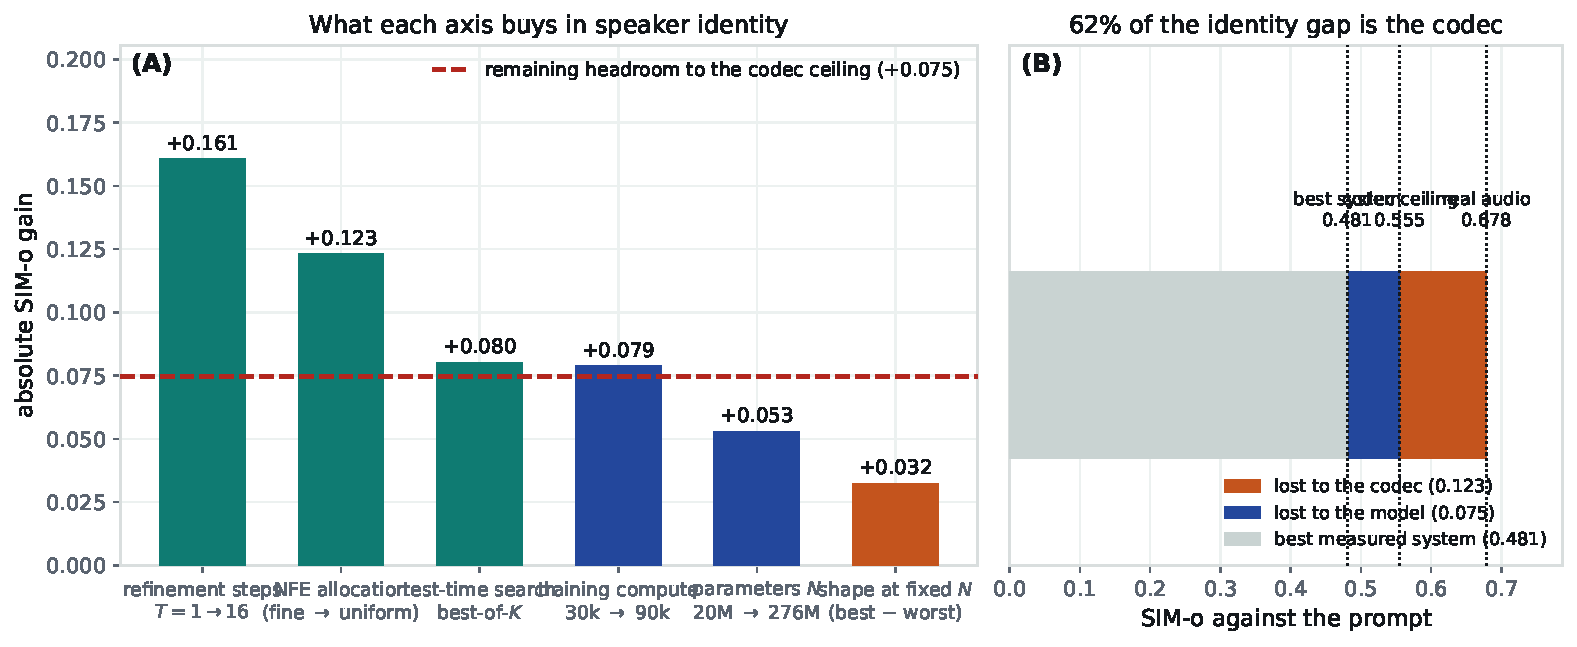
\includegraphics[width=\linewidth]{figures/identity_ledger.pdf}
  \caption{\textbf{(A)}~SIM-o gains of Table~\ref{tab:ledger}; search bars are ECAPA-selected and
  at matched NFE, refinement (faded) starts at $T{=}1$. \textbf{(B)}~\NcodecShare\% of the gap to real audio is
  lost in the Mimi codec.}
  \label{fig:ledger}
\end{figure}

\subsection{What else raises speaker similarity}
\label{sec:identity}
Apart from refinement itself, whose gain is counted from unusable one-step output, training
longer raises SIM-o most and adding parameters comes second; search and guidance gain much
less (Table~\ref{tab:ledger}, Fig.~\ref{fig:ledger}). Retraining three
configurations from 30k to 90k steps raises SIM-o by \NtrainGainSim\ (CI \NtrainGainCI,
\NtrainGainRuns\ runs), and, for one run (C3, seed 0), doubling again to 180k adds \NtrainDouble\ (CI over items
\NtrainDoubleCI). Moving from the best 20\,M shape to the best \NmaxNfour\,M shape at 30k steps
adds \NparamGainSim.

Speaker-contrastive guidance runs a second forward pass per step, so guided $T{=}16$ costs
NFE 256 and is compared with unguided $T{=}32$. At NFE 256, best-of-4 search with ECAPA
selecting gains \NcrXEWMidd\ over unguided $T{=}32$, and guidance at $\gamma{=}0.5$ gains
\NcrGuideGainSim\ (CI \NcrGuideGainCI). At matched NFE, search's gain grows with $K$:
\NcrXEWLod, \NcrXEWMidd\ and \NcrXEWHid\ at $K=2,4,8$ (Table~\ref{tab:search}). Raising
$\gamma$ does not help guidance: its gain is $\NcrGamMidsim$ at $\gamma{=}1.0$ and
$\NcrGamHisim$ at $\gamma{=}2.0$ (App.~\ref{app:interventions}). Guidance also costs
\NcrGuideWER\ WER points, above the registered limit of 2.0 points, so its registered test
(H-S4) fails (App.~\ref{app:prereg}).

Rate matching and longer prompts add little (App.~\ref{app:interventions}). Setting each
item's length from its own prompt's speaking rate gains \NrateGainSim. Prompts longer than
the 3\,s used in training do not raise SIM-o, and at 9\,s they raise WER by \NctxWerCost\
points. Finally, \NcodecShare\% of the distance between our best 90k-step model and real
audio is lost in the Mimi codec (Fig.~\ref{fig:ledger}B).
